\documentclass[letterpaper, 12pt]{math}

\usepackage{tikz}

\title{Multivariable and Vector Calculus}
\author{Alvin Lin}
\date{August 2017 - December 2017}

\begin{document}

\maketitle

\section*{Double Integrals}
Find the volume of a solid under \( z = f(x,y) \) where:
\[ (x,y)\in D \quad a\le x\le b \quad l(x)\le y\le u(x) \quad
  f(x,y)\ge 0\text{ for }f(x,y)\in D \]
\begin{center}
  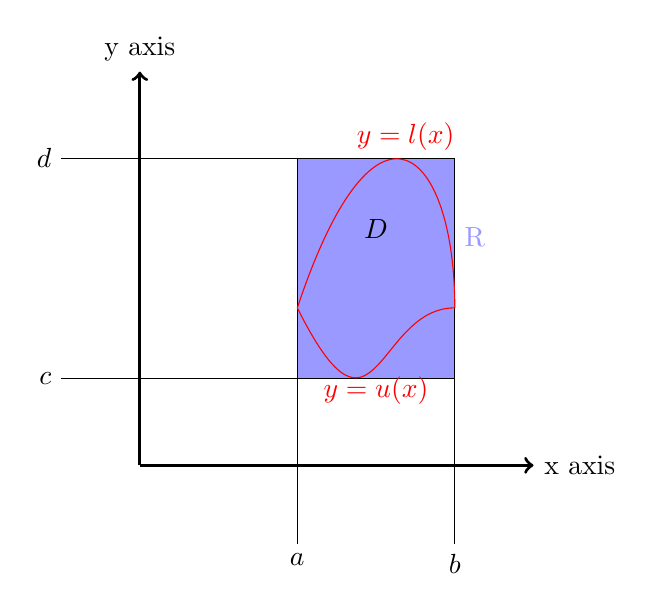
\begin{tikzpicture}
    \draw[very thick,->] (0,0) -- (5,0) node[right] {x axis};
    \draw[very thick,->] (0,0) -- (0,5) node[above] {y axis};
    \fill[blue!40!white] (2,1.1) rectangle (4,3.9) node[yshift=-1cm, right] {R};
    \draw (2,3.9) -- (2,-1) node[below] {\( a \)};
    \draw (4,3.9) -- (4,-1) node[below] {\( b \)};
    \draw (4,1.1) -- (-1,1.1) node[left] {\( c \)};
    \draw (4,3.9) -- (-1,3.9) node[left] {\( d \)};
    \node at (3,3) {\( D \)};
    \draw[red] (2,2) .. controls (3,0) and (3,2) .. (4,2) node[pos=0.5, below]
      {\( y = u(x) \)};
    \draw[red] (2,2) .. controls (3,5) and (4,4) .. (4,2) node[pos=0.5, above]
      {\( y = l(x) \)};
  \end{tikzpicture}
\end{center}
\[ D \subset R = [a,b]\times[c,d] \]
\[ V \approx |R|\cdot f(x_0,y_0), (x_0,y_0)\in D \]
This approximation is not very good. If we divide the region bounded by
\( [a,b] \) and \( [c,d] \) into \( n \) and \( m \) equal parts to form
\( R_{ij} \):
\[ V \approx \sum_{i=1}^{n}\sum_{i=1}^{m}|R_{ij}|f(x_{ij},y_{ij}) \]
This is the equivalent of a two dimensional Riemann sum.
\textbf{Theorem:} If \( z = f(x,y) \) is continuous for \( (x,y)\in D \),
\( y = l(x), y = u(x) \) are continuous for \( a\le x\le b \) then there
exists:
\[ \lim_{n,m\to0}\sum_{i=1}^{n}\sum_{i=1}^{m}|R_{ij}|f(x_{ij},y_{ij}) \]
which does not depend on the choice of points \( (x_{ij},y_{ij})\in R_{ij} \).
This limit is called the \textbf{double integral} of \( f(x,y) \) on D and
is equal to:
\[ \iint_{D}f(x,y)\diff{A} =
  \int_{a}^{b}\left[\int_{l(x)}^{u(x)}f(x,y)\diff{y}\right]\diff{x} \]

\subsubsection*{Example}
Find the volume of a solid under \( z = y^2, 0\le x\le4, 0\le y\le2 \). Give
the approximation of \( V \) when we divide \( [a,b] \) into 4 parts and
\( [c,d] \) into 2 parts, picking points in the middle for our Riemann sum.
\begin{center}
  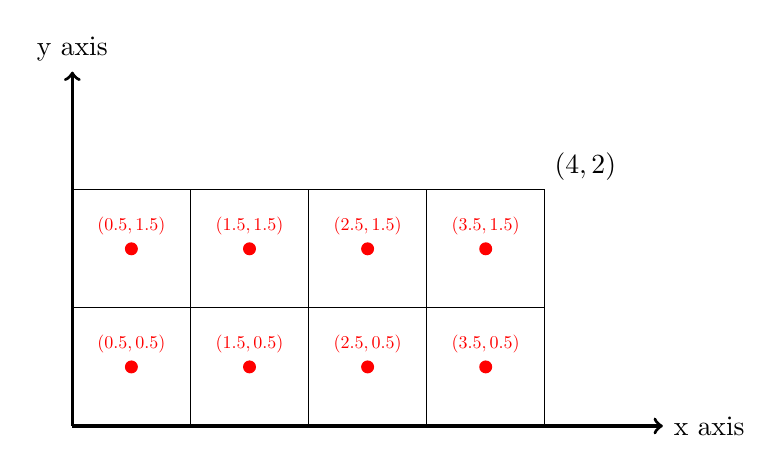
\begin{tikzpicture}[scale=1.5]
    \draw[very thick,->] (0,0) -- (5,0) node[right] {x axis};
    \draw[very thick,->] (0,0) -- (0,3) node[above] {y axis};
    \foreach \x in {1,2,3,4} {
      \draw (\x,0) -- (\x,2);
    };
    \foreach \y in {1,2} {
      \draw (0,\y) -- (4,\y);
    };
    \node[above right] at (4,2) {\( (4,2) \)};
    \foreach \x in {0.5,1.5,2.5,3.5} {
      \foreach \y in {0.5,1.5} {
        \draw[red, fill=red] (\x,\y) circle (0.05cm) node[above, yshift=0.1cm,
          scale=0.65] {\( (\x,\y) \)};
      }
    }
  \end{tikzpicture}
\end{center}
If we pick the center of each region (marked in red) as the approximation point:
\begin{align*}
  V &\approx
    1(\frac{1}{2})^2+1(\frac{1}{2})^2+1(\frac{1}{2})^2+1(\frac{1}{2})^2+
    1(\frac{3}{2})^2+1(\frac{3}{2})^2+1(\frac{3}{2})^2+1(\frac{3}{2})^2 \\
  &\approx 4(\frac{3}{2})^2+4(\frac{1}{2})^2 \\
  &\approx 10
\end{align*}
To find the exact volume:
\begin{align*}
  V &= \int_{0}^{4}\int_{0}^{2}y^2\diff{y}~\diff{x} \\
  &= \int_{0}^{4}\left[\frac{y^3}{3}\right]_0^2\diff{x} \\
  &= \int_{0}^{4}\frac{8}{3}\diff{x} \\
  &= \left[\frac{8}{3}x\right]_0^4 \\
  &= \frac{32}{3}
\end{align*}

\subsubsection*{Example}
Find the volume of the solid in the first octant bounded by \( 2x+y+z = 4 \).
\begin{align*}
  V &= \iint_{D}(4-2x-y)\diff{A} \\
  &= \int_{0}^{2}\left[\int_{0}^{4-2x}(4-2x-y)\diff{y}\right]\diff{x} \\
  &= \int_{0}^{2}\left[(4-2x)y-\frac{y^2}{2}\right]_0^{4-2x}\diff{x} \\
  &= \int_{0}^{2}(4-2x)^2-\frac{(4-2x)^2}{2}\diff{x} \\
  &= \int_{0}^{2}\frac{(4-2x)^2}{2}\diff{x} \\
  &= \left[\frac{1}{2}\frac{(4-2x)^3}{3}\frac{-1}{2}\right]_{0}^{2} \\
  &= \frac{4^3}{12} = \frac{16}{3}
\end{align*}

\subsubsection*{Example}
Find the volume of the solid bounded by \( x = z, y = x, x+y = 2, z = 0 \).
\begin{align*}
  V &= \iint_{D}x\diff{A} \\
  &= \int_{0}^{1}\left[\int_{x}^{2-x}x\diff{y}\right]\diff{x} \\
\end{align*}

\subsubsection*{Example}
Find the volume of the solid bounded by \( z = 3y, z = 2+y, y = x^2 \).
\begin{align*}
  V &= \iint_{D}2+y\diff{A}-\iint_{D}3y\diff{A} \\
  &= \iint_{D}2-2y\diff{A} \\
  &= \int_{-1}^{1}\left[\int_{x^2}^{1}(2-2y)\diff{y}\right]\diff{x}
\end{align*}

\subsubsection*{Example}
Evaluate:
\begin{align*}
  \int_{0}^{8}\int_{\sqrt[3]{y}}^{2}\e^{x^4}\diff{x}\diff{y} &=
    \int_{0}^{2}\left[\int_{0}^{x^3}\e^{x^4}\diff{y}\right]\diff{x} \\
  &= \int_{0}^{2}\left[\e^{x^4}y\right]_{0}^{x^3}\diff{x} \\
  &= \left[\e^{x^4}\frac{1}{4}\right]_{0}^{2}
\end{align*}

\begin{center}
  You can find all my notes at \url{http://omgimanerd.tech/notes}. If you have
  any questions, comments, or concerns, please contact me at
  alvin@omgimanerd.tech
\end{center}

\end{document}
